\documentclass{article}
\usepackage{url}
\usepackage{hyperref}
\usepackage{graphicx}
\usepackage{wrapfig}
\usepackage{listings}
\graphicspath{{./}}
\title{Taskmaster}
\author{
    Jotham Wong\\
    jw0771\\
    \and
    Chai Mauliola\\
    mauliola
}
\begin{document}
\maketitle

\section{Motivation}

Serverless computing or the Functions-as-a-Service (FaaS) paradigm is a rapidly growing cloud application model that sees popularity among startups and small-mid scale companies due to its advantage in blackboxing architectural constraints. However, it is plagued by a problem known as cold starts where time required to start up containers with their dependencies dominates. Chris Munns proposed that "pinging" a serverless function was really the only way to mitigate the issue of cold starts \cite{jeremydaly}.

\section{Methodology}

\subsection{Architecture}

\begin{figure}
    \begin{center}
        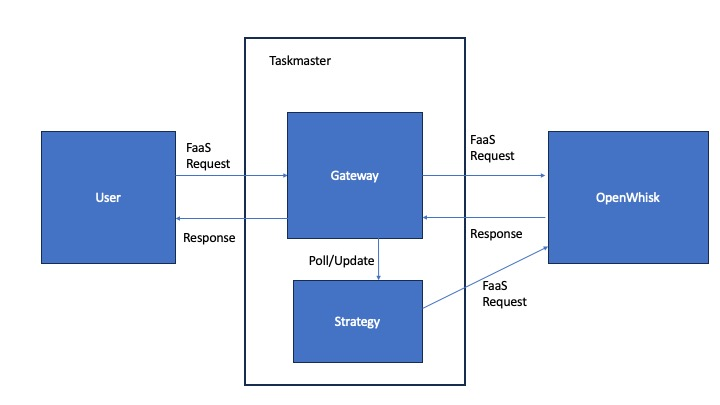
\includegraphics[width=\textwidth]{architecture.jpg}
    \end{center}
    \label{fig:taskmaster}
    \caption{Taskmaster architecture}
\end{figure}

The architecture of Taskmaster can be seen in Figure \ref{fig:taskmaster}. Taskmaster essentially consists of three components: 
\begin{enumerate}
    \item Gateway
    \item Strategy
    \item Openwhisk (FaaS framework)
\end{enumerate}

The FaaS framework used can be replaced by another FaaS framework since all FaaS frameworks have a cli tool available for creating and invoking actions, a simple modification can be made to the existing codebase to handle them appropriately. Openwhisk was chosen due to ease of use, it's architecture making use of docker containers which suffer from cold starts, exactly the problem we aim to investigate. From here onwards, we refer to Openwhisk as FaaS to make it clear that we don't rely on any Openwhisk specificities for Taskmaster's usage.

The Gateway is a standard HTTP server that sits between the user and the FaaS framework. Users invoke serverless function requests using a HTTP get request to the Taskmaster through the "/receive" route with their specified function name and parameters. The Gateway will route these requests to the FaaS framework and return the results if specified. The Gateway will also periodically poll the Strategy component at a specified interval (through the configuration file) and update the Strategy of function invocation patterns.

The Strategy is implemented as an interface that supports two methods: Update and Predict. In Update, it receives a key-value map of information that it can possibly use to update its internal state. When the Strategy is periodically polled by the Gateway, it will return a function name and parameters to the Gateway for "pinging" as mentioned by Chris Munns through its Predict method. Both Update and Predict are implementation dependent and any Strategy that satisfies this interface can be swapped by specifying the strategy in the configuration.

\subsection{Workloads}

To test our system, we artifically generate function request workloads using the python script "generator.py". Several probability distributions can be used to represent different patterns of workloads but we currently use the Gaussian distribution with a specified mean and variance to control the intervals at which the functions are invoked. We also create a testbed of serverless functions in the "functions" folder which range from simple hello world programs to slightly more complex functions in a wide variety of programming languages. The scripts are easily extensible to support testing on a wide range of scenarios.

\subsection{Strategy}\label{Strategy}

In this section, we detail the different strategies that were employed and provide experimental results in the next section.

\subsubsection{Naive}

We employ a periodicity of 0 which means that the Strategy is never called. This serves as our experimental baseline. Although this does incur some penalty due to the additional HTTP call that needs to be made, we assume that the delay is negligible in the context of containers shutting down with respect to the function invocation workload.

\subsubsection{LRU}

This Strategy resembles the LRU cache under the following intuition: a function container that was least recently used is most likely to shut down and subsequent function calls will incur the cold start penalty. Therefore, a simple linked list is used to maintain the LRU order and Update will update the internal LRU ordering. When the Strategy is polled, it will ping the lru function and move it back to the front of the queue.

\subsubsection{MRU}

This strategy is the same as the LRU strategy, except that the most recently used function will be kept alive. (note, this will likely be a redundant strategy, since its the same as the default strategy of scaling to zero after a set amout of time.)

\subsubsection{RS}

Random selection maintains a list of recently used functions and then keeps a randomly selected function warm.

\subsubsection{PQ}


\subsubsection{MFE}

Maintain a counter for each function and then ping the Most Frequently Encountered (MFE)

\section{Experimental Results}

For evaluation, we used the programming languages

\begin{enumerate}
    \item Java
    \item Javascript
    \item Php
    \item Ruby
    \item Python
\end{enumerate}

as well as simple functions that either had O(1) time complexity (the suite of Hello functions) as well as O(N) time complexity (the suite of factorial functions). This was to introduce some variance in the time it would take for the function completion. Golang was excluded from our testing suite as we ran into issues getting the go binary to execute on the serverless container. We generated our workload with the command and used this same test\_workload function for all experiments.

\begin{lstlisting}[language=bash,caption={Generating the workload}]
python generator.py test_workload 1000 5 1 functions_test 
\end{lstlisting}

For each strategy in \ref{Strategy}, we ran the simulation with polling periodicity set to 1, 5 and 10 seconds and measured the number of cold, prewarmed, warmed and recreated container states using Openwhisk's logs. We also ran an experiment with polling periodicity set to 0 to reflect the baseline wherein no strategy is used. The experimental results can be seen below.

TODO: Finish experiments, plot a table of cold, prewarmed, warmed and recreated container states in total as well as for each function.

\section{Conclusion and Further work}

In this research project, we have investigated the use of "pinging" serverless functions in an attempt to remedy the cold start problem and TODO: Add conclusion

Due to time limits, we were unable to add more complicated strategies that we initially had in mind, such as a ML forecasting approach that would train on the previous day's workload and use a Flask server as the endpoint for the prediction. We would also have explored a longer workload file with a larger suite of serverless functions lasting a full day instead of the current runtime of 1 hour 20 minutes for more realism in the experiments.

\section{Acknowledgements}

Thanks to Leo Chen for his feedback on improving our project scope.

\bibliography{ref.bib}
\bibliographystyle{acm}
\end{document}